\subsubsection{Image Analysis Techniques}
	There are a number of analysis techniques which can be applied to imagery to extract information. Perhaps the most common is analysing the pixels in an image to identify discontinuities in their data values which suggests the edge of an object, structure, or land mass. Such functionality is readily available on desktop image processing packages designed for amateur photographers \citep{photoshop}. But scientific and engineering applications of edge detection provide far greater levels of sensitivity helping isolate objects that can be subsequently measured with a high level of accuracy \citep{matlabedge}.
	\paragraph{Thresholding}
		Image thresholding is the most basic form of image segmentation \citep{haralock1991computer}. At its simplest this would entail taking a greyscale image, examining the intensity of each pixel and setting those below a certain threshold to black and those above it to white as shown in Figure \ref{fig:threshold} below. By thresholding an image, objects lose detail but their silhouettes become clearer making them more visible to object detection techniques.
		\begin{figure}[h!]
			\centering
			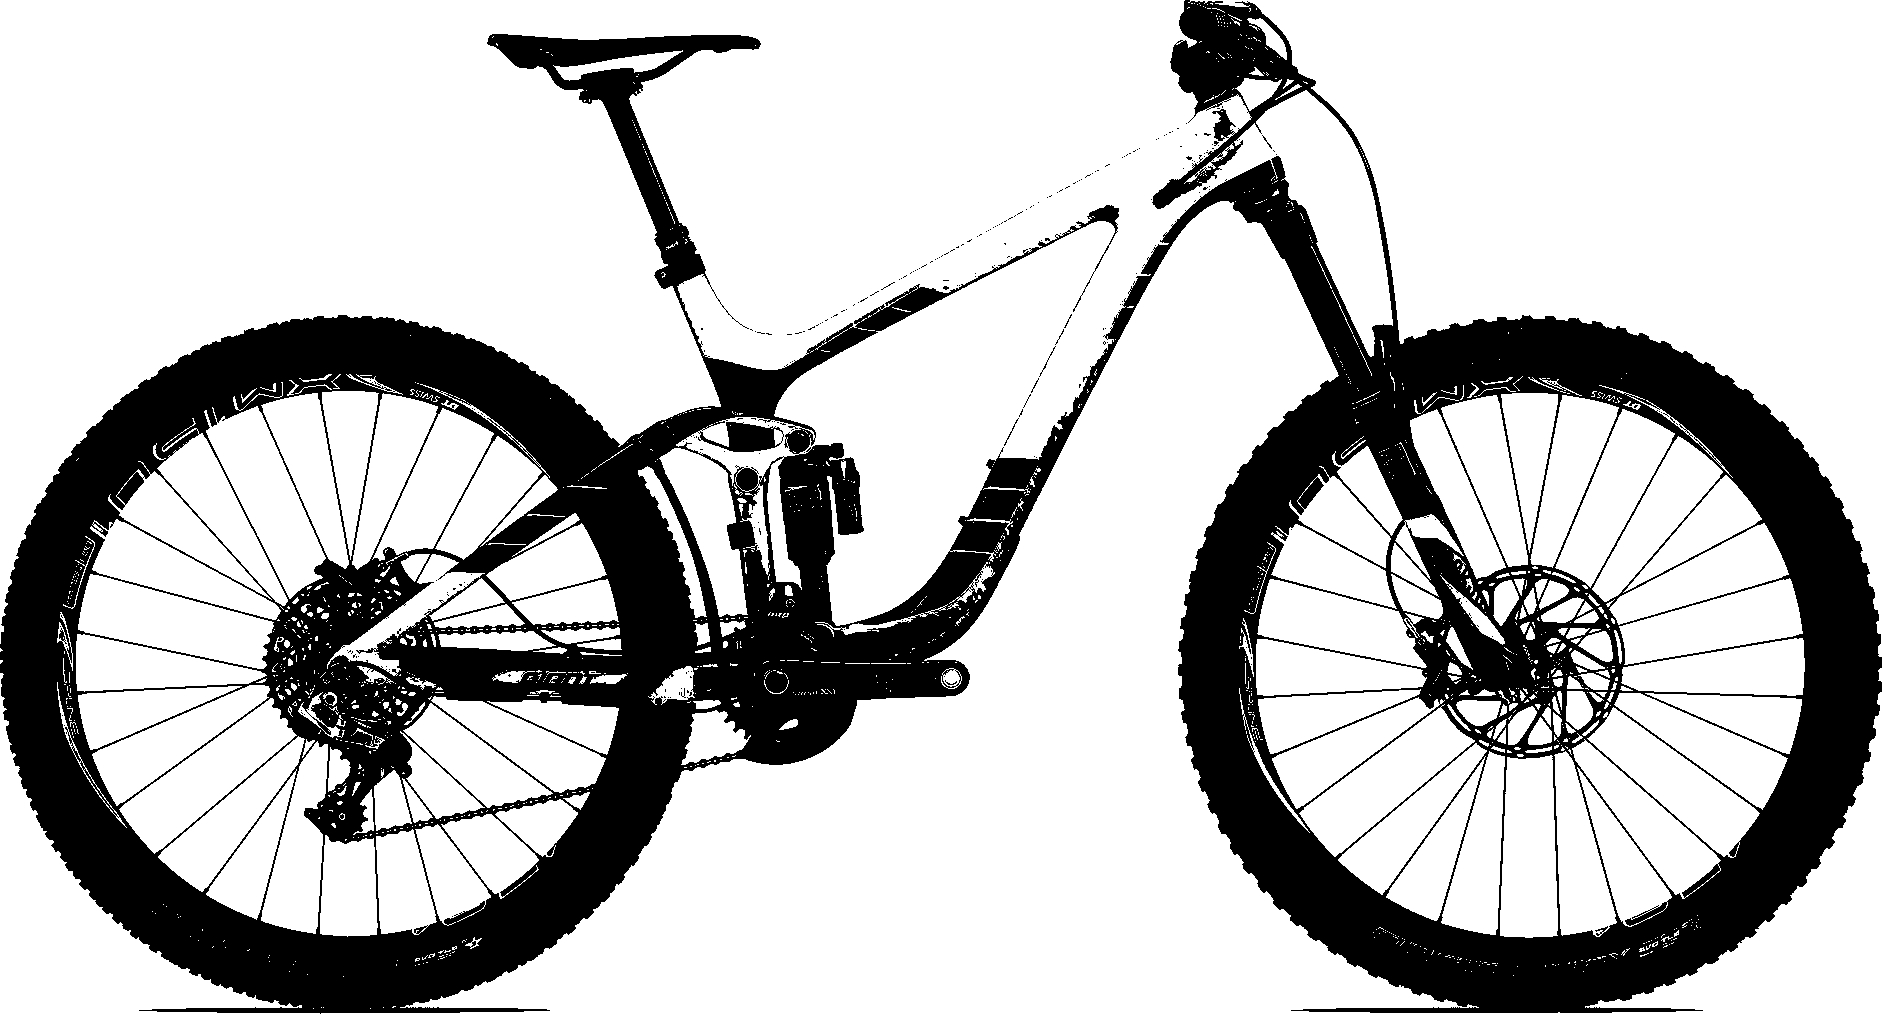
\includegraphics[width=8cm]{../images/reign_threshold.jpg}
			\caption{A copy of Figure \ref{fig:fsandht} with thresholding applied}
			\label{fig:threshold}
		\end{figure}
	\paragraph{Edge Detection}
		This is the application of mathematical algorithms to locate and highlight the edges of features in an image. There are multiple algorithms which can be used for edge detection, including Sobel, Roberts, Canny, and fuzzy logic, although all utilise the same basic concept of comparing the data values of adjacent pixels to find discontinuities from one value to another.
		\begin{table}[h!]
			\centering
			\caption{Table of pixel data showing an edge}
			\label{tab:edgePixels}
			\begin{tabular}{|c|c|c|c|c|c|c|}
				\hline
				5&7&6&4&152&148&149\\
				\hline
				\cellcolor[HTML]{0D0D0D}&
				\cellcolor[HTML]{121212}&
				\cellcolor[HTML]{0F0F0F}&
				\cellcolor[HTML]{0a0a0a}&
				\cellcolor[HTML]{989898}&
				\cellcolor[HTML]{949494}&
				\cellcolor[HTML]{959595}\\
				\hline
			\end{tabular}
		\end{table}\\
		Table \ref{tab:edgePixels} represents possible pixel values of an edge indicated by the large difference between 4 and 152. The applied algorithm will pick up this discontinuity which will be highlighted on the resulting image. A common application for edge detection is text recognition such as in automatic number plate recognition (ANPR) \citep{anpr} where edge detection is applied to highlight the block shapes of the vehicle registration plate. Figure \ref{fig:anpr} shows an image which has been edge detected with the number plate of the car clearly visible.
		\begin{figure}[h!]
			\centering
			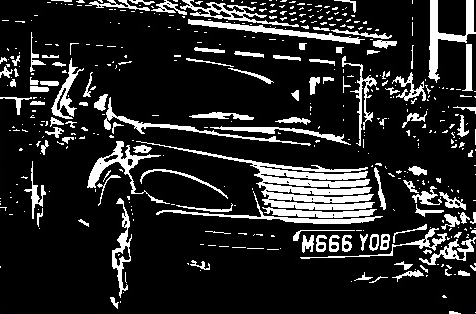
\includegraphics[width=10cm]{../images/anpr.jpg}
			\caption{Edge detection applied to an image for number plate recognition}
			\label{fig:anpr}
		\end{figure} 
	\paragraph{BLOB Analysis}
		\gls{blob} analysis is a method of feature detection used in image analysis \citep{introtoprocessing}. Typically carried out after thresholding, the pixels in an image are inspected and compared to their neighbours based on colour and intensity. If they are considered similar, the pixel locations are logged within some data structure which once complete will define all pixels within a single object.
		\\\\
		Once all \glspl{blob} are identified they can then be analysed based on some metric, which may be shape, colour, or size for example. What is done with the results of this is dependant on the project context though some uses include identification of pedestrians as shown in Figure \ref{fig:analysis_uses}, finding a reference point for measurements as explained in section \ref{sec:taking_measurements}, or reading characters in type \citep{blob}.		
	\paragraph{Hough Transform}\label{sec:lit_review_hough}
		Originally created in 1962 by Paul Hough, the Hough transform methods offer techniques for the discovery of imperfect objects in images. The original algorithms were created for the detection of lines but have since been improved and adapted to find circles, ellipses, and other basic shapes. 
		\\\\
		While edge detection is suitable for highlighting critical points in an image, it can be problematic if the base image is not well lit or out of focus causing an edge detector to produce imperfect lines. Such artefacts can make rudimentary feature detection techniques difficult but the Hough Transformation techniques circumvent such issues by considering points as a part of an object through a voting procedure.
		\\\\
		The collection of Hough transform algorithms are separated by the objects which they are capable of finding, such as linear Hough transform or circular Hough transform, and have been well described by \cite{hough}. The Hough transform methods could be used in this project for the detection of suspension units in images or sections of the whole bike depending on the chosen process for the application.	
	\paragraph{Taking Measurements}\label{sec:taking_measurements}
		To measure the dimensions of an object in an image, certain data about the camera and its location are required. By using digital imagery, the majority of this information is automatically provided as each image contains metadata or EXchangeable Image Format (EXIF) data which includes information such as camera manufacturer, focal length, image size, and location if available.
	\begin{equation}
		\label{equ:measureobj}
		H_{o} = \Bigg(\frac{f\times\big(\frac{H_{i}}{H_{s}}\big)}{D - f}\Bigg)\times H_{c}
	\end{equation}
	\begin{where}
		\item $f$~~~~is the focal length of the camera lens
		\item $D$~~~is the distance to the object
		\item $H_{o}$~~is the height of the object
		\item $H_{i}$~~is the height of the image in pixels
		\item $H_{s}$~~is the height of the camera sensor
		\item $H_{c}$~~is the height of the camera from the ground
	\end{where}
	\vspace{5mm}
	The process to calculate the height of an object in an image is shown in Equation \ref{equ:measureobj}. Necessary data, such as $f$, $H_i$, and $H_s$ can be acquired from EXIF data. However $D$ and $H_c$ are not collected by the camera and must be measured. When dealing with image analysis this means that this data has to be collected at the time the image is taken. To briefly test this equation, data was manufactured for each parameter and passed through the equation. This process was then reversed using the now known object height to see if the result matched the manufactured one, which it did.
	\\\\
	To circumvent using this equation, a reference object of a known size can be included in the image. This removes the need to consult EXIF data meaning objects can be measured, irrespective of the camera used, though IA techniques. The previously mentioned Mars rover, Curiosity, carries a United States penny and charts as reference objects so that its cameras can be precisely calibrated as shown in Figure \ref{fig:curiosity_calibration_chart}.
	\begin{figure}[h!]
		\centering
		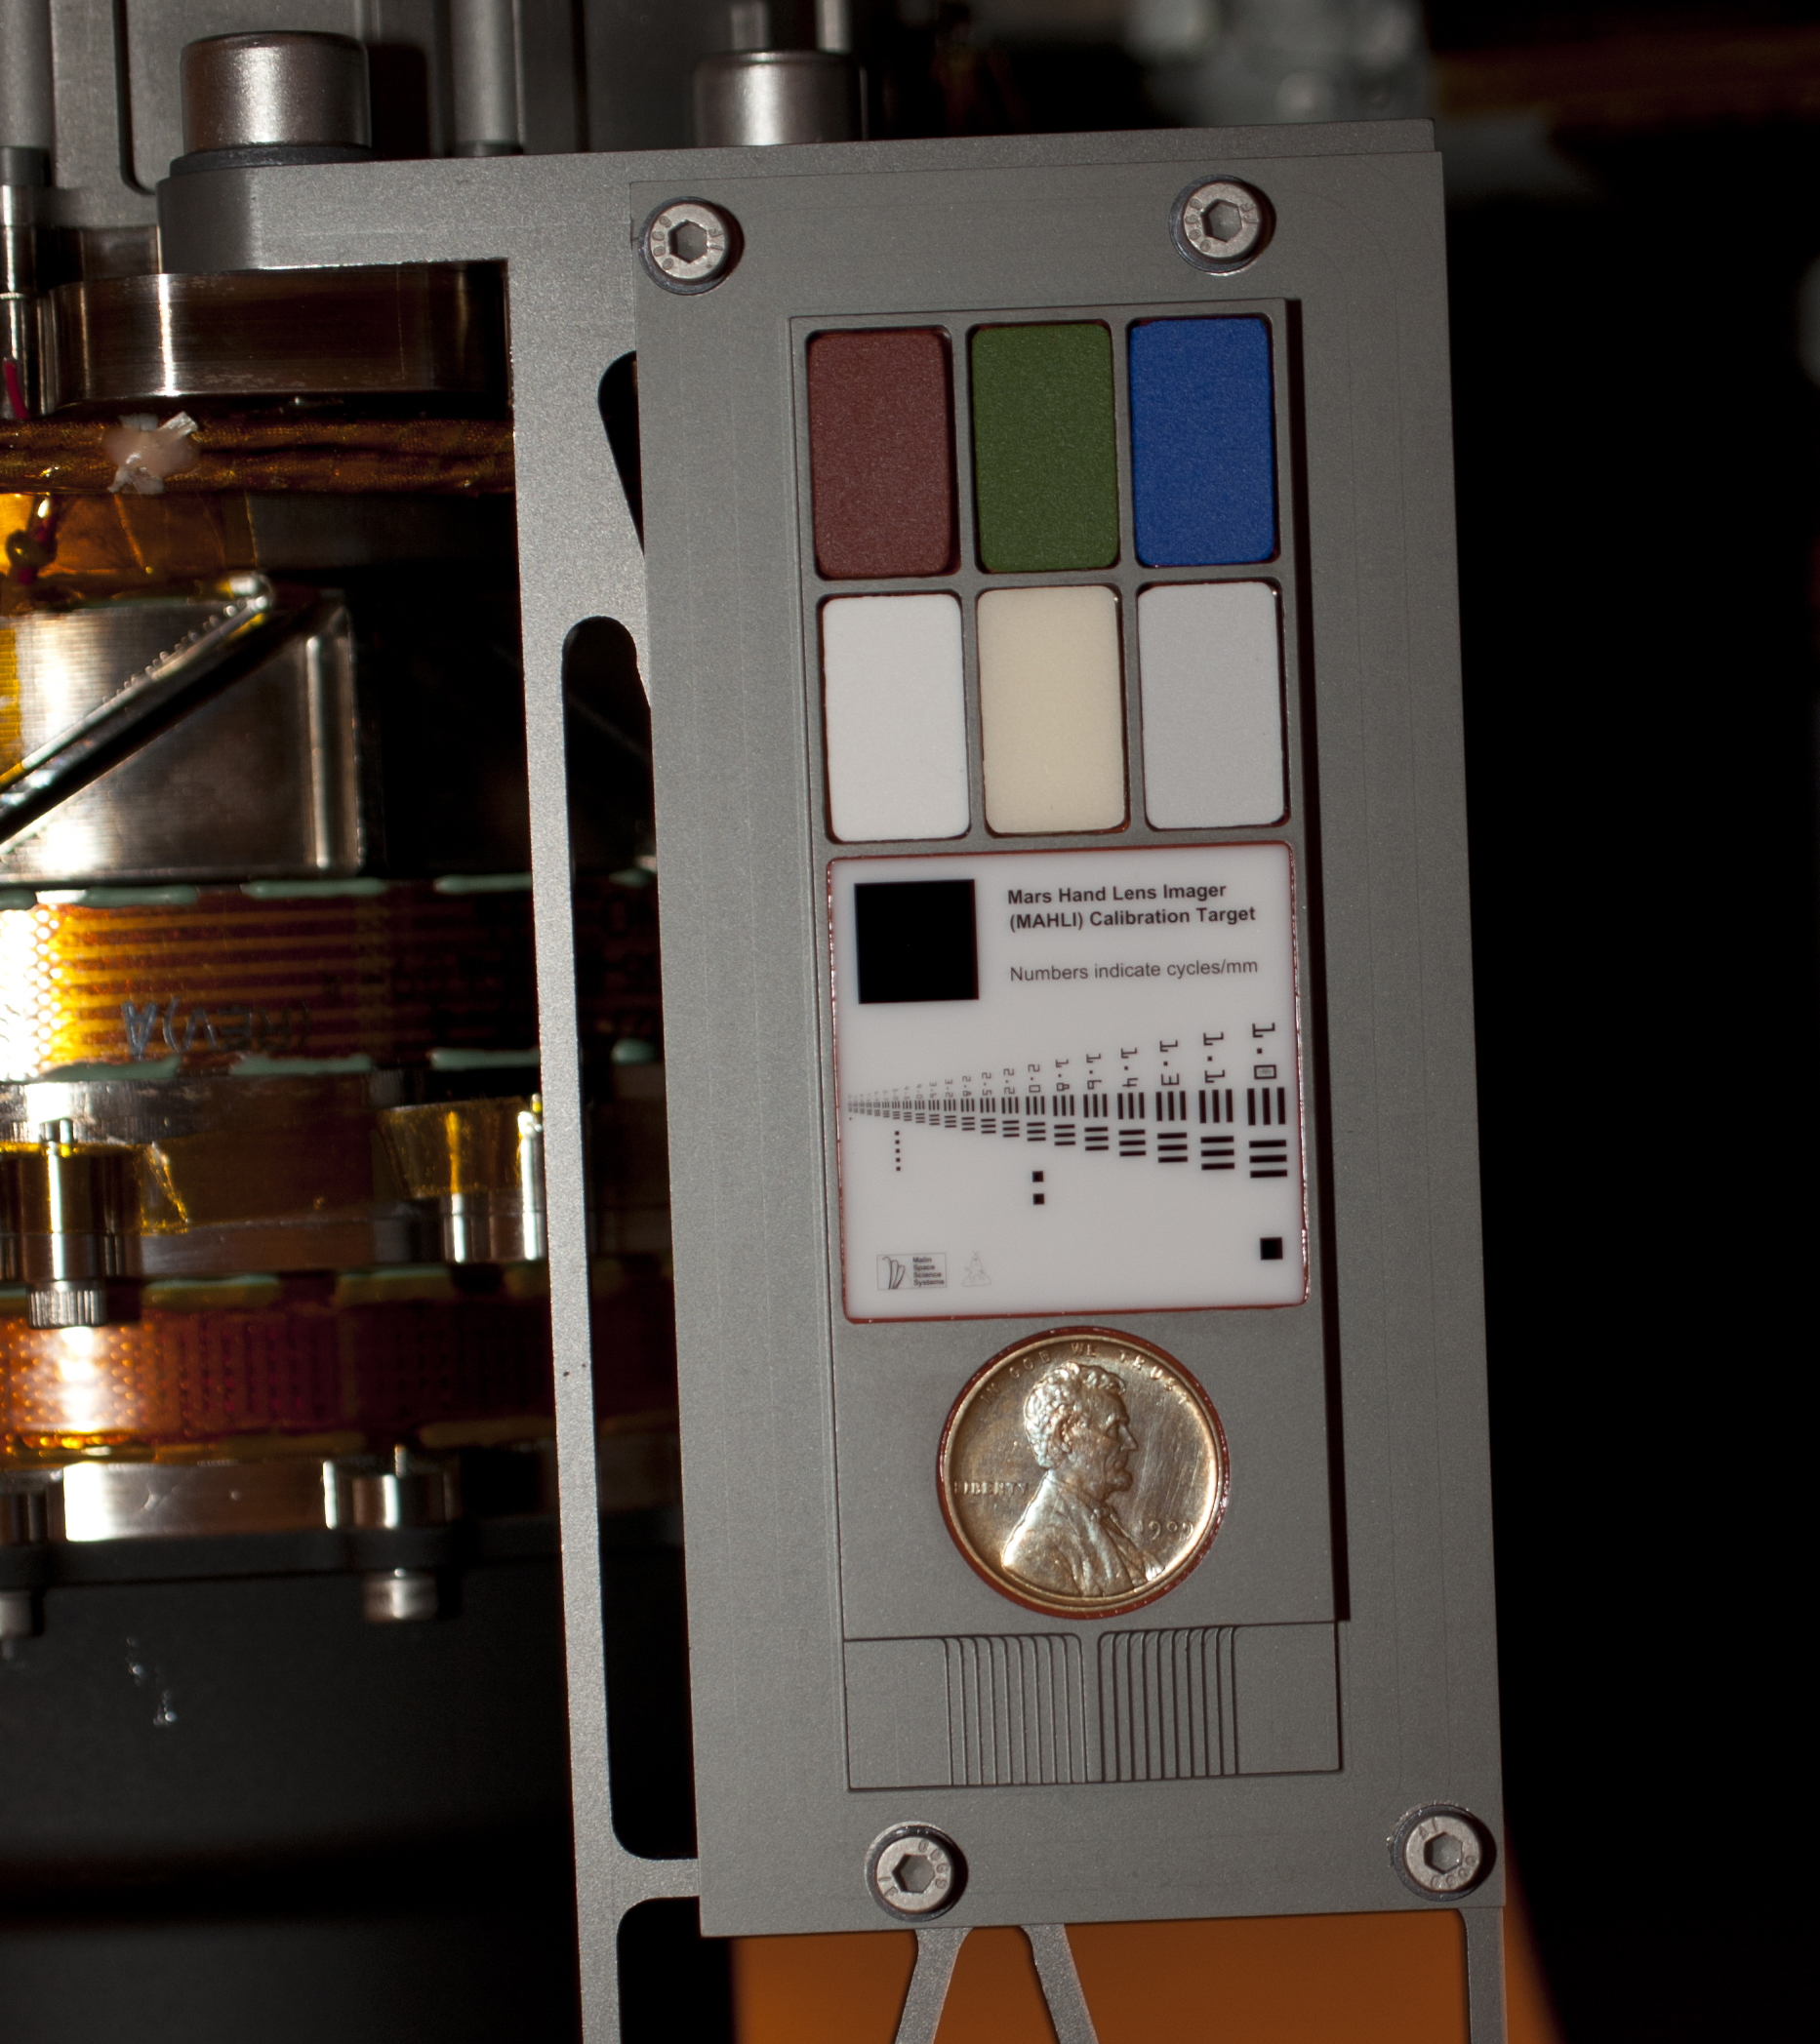
\includegraphics[width=7cm]{../images/curiosity_calibration_chart.jpg}
		\caption[Contact Instrument Calibration Targets on Mars Rover Curiosity]{Contact Instrument Calibration Targets on Mars Rover Curiosity \citep{curiosity_image_calibration}}
		\label{fig:curiosity_calibration_chart}
	\end{figure}\\\\
	First, the reference object must be located in the image using a technique such as \gls{blob} analysis or Hough transforms. Once the object is found, its width or height in pixels in the image is collected and compared against its actual size. This gives a ratio for applying to the pixel count of any object in the image to calculate its real world height. For example, if a reference object that is 2mm wide measures 200 pixels across in an image then it can be concluded that 100 pixels in the image corresponds to 1mm in the real world. If another object in the image measures 300 pixels across then it must be 3mm in the real world. This can only be concluded if the reference object and measurable object are of similar distance from the camera as perspective commonly causes issues when comparing the size of objects.
	\\\\
	This process will be applied during this project in some manner. Either a reference object will be used or the equation to calculate the height of an object will be applied. While incorporating Equation \ref{equ:measureobj} in an application will be relatively simple, collecting the necessary data without too much user interaction may be more difficult.